
\chapter{Matched-Pairs Experiment}
 \label{chapter::mpe}
 
The matched-pairs experiment (MPE) is the most extreme version of the SRE with only one treated unit and one control unit within each stratum. In this case, the strata are also called pairs. Although this type of experiment is a special case of the SRE discussed in Chapter \ref{chapter::stratification-poststratification}, it has its own estimation and inference strategy. Moreover, it has many new features and it is closely related to the ``matching'' strategy in observational studies which will be covered in Chapter \ref{chapter::matching-obs} later. So we discuss the MPE here,  in its own chapter. 





\section{Design of the experiment and potential outcomes}
 
Consider an experiment with $2n$   units. If we have predictive covariates to the outcomes, we can pair units based on the similarity of covariates. With a scalar covariate, we can order units based on this covariate and then form pairs based on the adjacent units. With many covariates, we can define pairwise distances between units and then form pairs based on these distances. In this case, pair matching can be done using a greedy algorithm or an optimal nonbipartite matching algorithm. The greedy algorithm pairs the two units with the smallest distance, drops them from the pool of units, pairs the two remaining units with the smallest distance, etc. The optimal nonbipartite matching algorithm divides the $2n$ units into $n$ pairs of two units to minimize the sum of the within-pair distances. See \citet{greevy2004optimal} for more details of the computational aspect of the MPE. In this chapter, we assume that the pairs are formed based on the covariates, and discuss the subsequent design and analysis issues. 


 Let $(i,j)$ index the unit $j$ in pair $i$, where $i=1,\ldots, n$ and $j=1,2$. Unit $(i, j)$  has potential outcomes $Y_{ij}(1)$ and $Y_{ij}(0)$ under the treatment and control, respectively. Within each pair, we randomly assign one unit to receive the treatment and the other to receive the control. Let
$$
Z_i = \begin{cases}
   1,& \text{if the first unit receives the treatment}, \\
   0, & \text{if the second unit receives the treatment}. 
\end{cases}  
$$ 
We can formally define MPE based on the treatment assignment mechanism. 


\begin{definition}
[MPE]
We have 
\begin{eqnarray}
 (Z_i)_{i=1}^n \iidsim \text{Bernoulli}(1/2).
 \label{eq::mp-treatment}
\end{eqnarray} 
\end{definition}

 
 
The observed outcomes within pair $i$ are 
$$
Y_{i1} = Z_i Y_{i1}(1) + (1-Z_i) Y_{i1}(0)
= \begin{cases}
   Y_{i1}(1),& \text{if } Z_i = 1; \\
   Y_{i1}(0), & \text{if } Z_i = 0; 
\end{cases}
$$
and
$$
Y_{i2} = Z_i Y_{i2}(0) + (1-Z_i) Y_{i2}(1)
= \begin{cases}
   Y_{i2}(0),& \text{if } Z_i = 1; \\
   Y_{i2}(1), & \text{if } Z_i = 0 . 
\end{cases} 
$$
So the observed data are $( Z_i, Y_{i1} , Y_{i2} )_{i=1}^n$.  
 
 
\section{FRT}
 
 Similar to the discussion before, we can always use the FRT to test the sharp null hypothesis: 
$$
\HF: Y_{ij}(1) = Y_{ij}(0)  \text{ for all }  i=1,\ldots  n  \text{ and } j=1,2. 
$$
When conducting the FRT, we need to simulate the distribution of $(Z_1, \ldots, Z_n)$ from \eqref{eq::mp-treatment}. 
I will discuss some canonical choices of test statistics based on the within-pair differences between the treated and control outcomes:
\begin{eqnarray*}
\hat{\tau}_i &=& \text{outcome under treatment} - \text{outcome under control} \text{ (within pair } i) \\
&=&  (2Z_i - 1) (Y_{i1}  - Y_{i2})\\
&=& S_i (Y_{i1}  - Y_{i2})  , 
\end{eqnarray*}
where the $S_i = 2Z_i - 1$ are IID random signs with mean $0$ and variance $1$, for $i=1,\ldots, n$. 
 Since the pairs with zero $\hat{\tau}_i $'s do not contribute to the randomization distribution, we drop those pairs in the discussion of the FRT. 
 
\begin{example} 
[paired $t$ statistic]\label{eg::paired-t-statistic}
The average of the within-pair differences is
$$
\hat{\tau} = n^{-1}  \sumn \hat{\tau}_i .
$$
Under $\HF$, 
$$
E(\hat{\tau} ) = 0
$$
and
$$
\var(  \hat{\tau}   ) 
= n^{-2} \sumn \var(  \hat{\tau}_i ) 
= n^{-2} \sumn \var(S_i) (Y_{i1}  - Y_{i2})^2 =  n^{-2} \sumn  \hat{\tau}_i^2 . 
$$
Based on the CLT for the sum of independent random variables, we have the  Normal approximation:
$$
\frac{  \hat{\tau}  }{ \sqrt{  n^{-2} \sumn  \hat{\tau}_i^2 } } \rightarrow \N01 
$$
in distribution.  We can use this Normal approximation to construct an asymptotic test. Many standard textbooks suggest using the following paired $t$ statistic in the MPE:
$$
t_\text{pair} = \frac{  \hat{\tau}  }{ \sqrt{  \{ n(n-1) \}^{-1} \sumn  (\hat{\tau}_i - \hat{\tau} ) ^2 } },
$$
which is almost identical to $\hat{\tau}$ with large $n$ and small $\hat{\tau} $ under $\HF$. 
\end{example} 

In classic statistics, the motivation for using $t_\text{pair}$ is under a different framework. When $\hat{\tau}_i \iidsim \textsc{N}(0, \sigma^2)$, we can show that $t_\text{pair} \sim t(n-1)$, i.e., the exact distribution of $t_\text{pair} $ is $t$ with degrees of freedom $n-1$, which is close to $\N01$ with a large $n$. The \ri{R} function \ri{t.test} with \ri{paired=TRUE} can implement this test. With a large $n$, these procedures give similar results. The discussion in Example  \ref{eg::paired-t-statistic} gives another justification of the classic paired $t$ test without assuming the Normality of the data. 

 
 
 

 
 
  \begin{example}
 [Wilcoxon sign-rank statistic]\label{eg::mpe-sign-rank}
Based on the ranks $(R_1, \ldots, R_n)$ of $( | \hat{\tau}_1| , \ldots, | \hat{\tau}_n| )$, we can define a test statistic
$$
W = \sumn  I( \hat{\tau}_i > 0 ) R_i. 
$$
%Under $\HF$, we can drop the pairs with $ \hat{\tau}_i = 0$ since those pairs do not contribute to the randomization distribution of $W$. Ignoring those pairs with $ \hat{\tau}_i = 0$, we 
Under $\HF$, the $| \hat{\tau}_i|$'s are fixed so the $R_i$'s are also fixed, which implies that 
$$
E(W) = \frac{1}{2} \sumn R_i = \frac{1}{2} \sumn i = \frac{n(n+1)}{4}
$$
and
$$
\var(W) = \frac{1}{4} \sumn R_i^2 = \frac{1}{4} \sumn i^2 = \frac{n(n+1)(2n+1)}{24}. 
$$
The CLT for the sum of independent random variables ensures the following Normal approximation: 
$$
\frac{W - n(n+1)/4}{ \sqrt{n(n+1)(2n+1) / 24    } } \rightarrow \N01
$$
in distribution. 
We can use this Normal approximation to construct an asymptotic test.  The \ri{R} function \ri{wilcox.test} with \ri{paired=TRUE} can implement both the exact and asymptotic tests. 
 \end{example}
 
 
 
 
   \begin{example}
 [Kolmogorov--Smirnov-type statistic]\label{eg::mpe-ksstatistics}
Under $\HF$, the absolute values $( | \hat{\tau}_1| , \ldots, | \hat{\tau}_n| )$ are fixed but their signs are random. So $   (  \hat{\tau}_1 , \ldots,  \hat{\tau}_n  )$ and $ -   (  \hat{\tau}_1 , \ldots,  \hat{\tau}_n  )$ should have the same distribution. 
Let 
$$
\hat{F}(t)  = n^{-1} \sumn I( \hat{\tau}_i  \leq t  )
$$
be the empirical distribution of $  (  \hat{\tau}_1 , \ldots,  \hat{\tau}_n  )$, and
$$
1 - \hat{F}(-t-)  =    n^{-1} \sumn I( -  \hat{\tau}_i  \leq t  )
$$ 
be the empirical distribution of $ -   (  \hat{\tau}_1 , \ldots,  \hat{\tau}_n  )$, where $\hat{F}(-t-)$ is the left limit of the function $\hat{F}(\cdot)$ at $-t$. 
A Kolmogorov--Smirnov-type statistic is then 
$$
D = \max_t |  \hat{F}(t)  +  \hat{F}(-t-)  - 1  |.
$$
\citet{butler1969test} proposed this test statistic and derived its exact and asymptotic distributions. Unfortunately, this is not implemented in standard software packages. Nevertheless, we can simulate its exact distribution and compute the $p$-value based on the FRT. \footnote{
\citet{butler1969test}'s proposed this test statistic under a slightly different framework. Given IID draws of $    (  \hat{\tau}_1 , \ldots,  \hat{\tau}_n  )$ from a  distribution $F(y)$, if they are symmetrically distributed around $0$, then
$$
F(t) = \pr( \hat{\tau}_i \leq t ) =  \pr( -  \hat{\tau}_i \leq t )  = 1 - \pr( \hat{\tau}_i <- t) = 1 - F(-t-).
$$
Therefore, $\hat{F}(t)  +  \hat{F}(-t-)  - 1 $ measures the deviation from the null hypothesis of symmetry, which motivates the definition of $D$ in Example \ref{eg::mpe-ksstatistics}. A naive definition of the Kolmogorov--Smirnov-type statistic is to compare the empirical distributions of the outcomes under treatment and control as in Example \ref{eg::ks-CRE}. Using that definition, we effectively break the pairs. Although it can still be used in the FRT for the MPE, it does not capture the matched-pairs structure of the experiment.}
 \end{example}
 
 
 
 
 
  \begin{example}
 [sign statistic]\label{eg::mpe-sign}
 The sign statistic uses only the signs of the within-pair differences
 $$
 \Delta = \sumn I( \hat{\tau}_i > 0 ).
 $$
% Again the pairs with $\hat{\tau}_i = 0$ do not contribute to the randomization distribution of $ \Delta $, so we drop them without loss of generality. 
 Under $\HF$, 
 $$
 I( \hat{\tau}_i > 0 ) \iidsim \textup{Bernoulli}(1/2)
 $$
 and therefore 
 $$
  \Delta \sim \textup{Binomial}(n, 1/2).
 $$
 Based on this we have an exact Binomial test, which is implemented in the \ri{R} function 
\ri{binom.test} with \ri{p=1/2}. Using the CLT, we can also conduct a test based on the following Normal approximation of the Binomial distribution: 
$$
\frac{  \Delta - n/2 }{  \sqrt{n/4} } \rightarrow \N01 
$$
in distribution. 
 \end{example}
 
 
 
 \begin{example}
 [McNemar's statistic for a binary outcome]\label{eg::mcnenar-test-binary}
 If the outcome is binary, we can summarize the observed data from the MPE in a more compact way. Given a pair, the treated outcome can be either $1$ or $0$ and the control outcome can be either $1$ or $0$, yielding a two-by-two table as in Table \ref{tb::binarymatchedpairs}. 
 
\begin{table}
\centering
\caption{Counts of four types of pairs}\label{tb::binarymatchedpairs}
\begin{tabular}{ccc}
\hline 
 & control outcome 1 & control outcome 0\\
 \hline 
treated outcome 1 & $m_{11}$ & $m_{10}$ \\
treated outcome 0 & $m_{01}$ & $m_{00}$ \\
\hline 
\end{tabular}
\end{table} 
 
Under $\HF$, the numbers of concordant pairs $m_{11}$ and $m_{00}$ are fixed, and $m_{10} + m_{01}$ is also fixed. So the only random component is $m_{10}$ which has distribution 
$$
m_{10} \sim \textup{Binomial}( m_{10} + m_{01}, 1/2  ).
$$ 
This implies an exact test based on the Binomial distribution. The \ri{R} function \ri{mcnemar.test} gives an asymptotic test based on the Normal approximation of the Binomial distribution:
$$
\frac{   m_{10}  - (m_{10} + m_{01})/2  }{  \sqrt{  (m_{10} + m_{01}) / 4   } } 
= \frac{ m_{10}  -  m_{01}   }{  \sqrt{ m_{10} + m_{01}    }  }
\rightarrow \N01  
$$
in distribution. Both the exact FRT and the asymptotic test do not depend on $m_{11}$ or $m_{00}$. Only the numbers of discordant pairs matter in these tests. 
 \end{example}
 
 
 
\section{Neymanian inference}
 
The average causal effect within pair $i$ is 
 $$
 \tau_i = \frac{1}{2}  \left\{    Y_{i1}(1) + Y_{i2}(1) -     Y_{i1}(0)  - Y_{i2}(0)     \right\},
 $$
 and the average causal effect for all units is
$$
\tau = n^{-1} \sumn  \tau_i  = (2n)^{-1} \sumn \sum_{j=1}^2 \{  Y_{ij}(1) - Y_{ij}(0)   \} .
$$
It is intuitive that  $\hat{\tau}_i $ is unbiased for $ \tau_i $, so $\hat{\tau}  $ is unbiased for $\tau$. We can also calculate the variance of $\hat{\tau}  $. I relegate the exact formula to Problem \ref{para::variance-mp-design}  because the MPE is just a special case of the SRE. 


However, we cannot follow the strategy under the SRE to estimate the variance of $\hat{\tau}  $ under the MPE. The within-pair sample variances of the outcomes are not well defined because, within each pair, we have only one treated and one control unit. The data do not allow us to estimate the variance of $\hat{\tau}_i $ within pair $i$.  


Is it possible to estimate the variance of $\hat{\tau}$ in the MPE? Let us forget about the MPE and change the perspective to the classic IID sampling. If the $\hat{\tau}_i$'s are IID with mean $\mu$ and $\sigma^2$, then the variance of $\hat{\tau} = n^{-1} \sumn \hat{\tau}_i$ is $\sigma^2 / n$. An unbiased estimator for $\sigma^2$ is the sample variance $(n-1)^{-1} \sumn ( \hat{\tau}_i -  \hat{\tau} )^2$, so an unbiased estimator for $\var( \hat{\tau}  )$ is 
\begin{equation}\label{eq::mpe-variance-estimation}
\hat{V} = \{ n(n-1)  \}^{-1} \sumn ( \hat{\tau}_i -  \hat{\tau} )^2.
\end{equation}
The discussion also extends to the independent but not IID setting; see Problem \ref{hw::inid} in Chapter \ref{chapter::basic-prob-append}.
The above discussion seems a digression from the MPE which has completely different statistical assumptions. But at least it motivates a variance estimator $\hat{V} $, which uses the between-pair variance of $\hat{\tau}_i $ to estimate the variance of $\hat{\tau}  $.  Of course, it is derived under different assumptions. Does it also work for the MPE? Theorem \ref{thm::varianceest-mp} below is a positive result.
 
\begin{theorem}\label{thm::varianceest-mp}
Under the MPE, $\hat{V}$ defined in \eqref{eq::mpe-variance-estimation} is a conservative estimator for the true variance of $\hat{\tau}  $:
$$
E(  \hat{V}) - \var(   \hat{\tau}  ) = \{ n(n-1)  \}^{-1} \sumn  (\tau_i - \tau)^2 \geq 0  .
$$
If the $\tau_i$'s are constant across pairs, then $E(  \hat{V} )  = \var(\hat{\tau}) .$
\end{theorem}


Theorem \ref{thm::varianceest-mp} states that under the MPE, $\hat{V} $ is a conservative variance estimator in general and becomes unbiased if the average causal effects are constant across pairs. It is somewhat surprising because $\hat{V} $ depends on the between-pair variance of the $ \hat{\tau}_i $'s whereas $ \var(   \hat{\tau}  ) $ depends on the within-pair variance of each of $ \hat{\tau}_i $. The proof below might provide some insights into this surprising result. 
 
 


\begin{myproof}{Theorem}{\ref{thm::varianceest-mp}}
Recall the basic algebraic fact that $\sumn (a_i - \bar a)^2 = \sumn a_i^2 - n \bar{a}^2$ which parallels the fact that $\var(W) = E(W^2) - (EW)^2$ for a random variable $W$. Use it in the following steps 2 and 5, we have 
\begin{eqnarray*}
n(n-1) E( \hat{V} ) &=& E\left\{   \sumn (\hat{\tau}_i - \hat{\tau})^2 \right\}  \\
&=&  E\left (    \sumn \hat{\tau}_i^2 - n \hat{\tau}^2  \right)   \\
&=& \sumn \{  \var(\hat{\tau}_i) + \tau_i^2 \} - n \{  \var(\hat{\tau})  + \tau^2 \}\\
&=& \sumn  \var(\hat{\tau}_i)  - n \var(\hat{\tau}) + \sumn  \tau_i^2 - n  \tau^2 \\
&=& n^2 \var(\hat{\tau})  - n \var(\hat{\tau})  + \sumn (\tau_i - \tau)^2.
\end{eqnarray*}
Therefore,
$$
E( \hat{V} )  = \var(\hat{\tau})  + \{ n(n-1)  \}^{-1}   \sumn (\tau_i - \tau)^2 \geq  \var(\hat{\tau})  .
$$
\end{myproof}




Similar to the discussions for other experiments, the Neymanian approach relies on the large-sample approximation:
$$
\frac{  \hat\tau  -  \tau }{  \sqrt{\var( \hat\tau )} } \rightarrow \N01
$$
in distribution if $n\rightarrow \infty$ and some regularity conditions hold. Due to the over-estimation of the variance, the Wald-type confidence interval
$$
 \hat\tau   \pm     z_{1-\alpha/2}  \sqrt{ \hat{V} }
$$
covers $\tau$ with probability at least $1-\alpha$.



Both the point estimator $\hat\tau$ and the variance estimator $\hat{V}$ can be conveniently obtained by OLS, as shown in the proposition below. 

\begin{proposition}\label{prop::mpe-variance}
$\hat\tau$ and
$\hat{V}$ are identical to the coefficient and variance estimator of the intercept from the OLS fit of the vector $(\hat{\tau}_1, \ldots, \hat{\tau}_n)\tran$ on the intercept only.
\end{proposition}

  I leave the proof of Proposition \ref{prop::mpe-variance} as Problem \ref{para::seols-matchedpairs}. 
  
  

\section{Covariate adjustment}



Although we have matched on covariates in the design stage, it is possible that the matching is not perfect $(X_{i1}\neq X_{i2})$ and sometimes we have additional covariates beyond those used in the pair-matching stage. In those cases, we can adjust for the covariates to further improve estimation efficiency. Assume that each unit $(i, j)$ has covariates $X_{ij} $. Similar to the discussion in the CRE, there are two general strategies of covariate adjustment in the MPE. 



\subsection{FRT}

 
I start with the covariate-adjusted FRT in the MPE. In parallel with Definition \ref{def::pseudo-y-frt},  we can construct test statistics based on the residuals from a model fitting of the outcome on the covariates, since those residuals are fixed numbers under the sharp null hypothesis. A canonical choice is to fit OLS of all observed $Y_{ij}$'s on $X_{ij}$'s to obtain the residuals $\hat \varepsilon_{ij}$'s. We can then construct test statistics pretending that the $\hat \varepsilon_{ij}$'s are the observed outcomes. \citet{rosenbaum2002covariance} advocated this strategy in particular to the MPE. 


In parallel with Definition \ref{def::model-out-frt}, we can directly use some coefficients from model fitting as the test statistics. The discussion in the next subsection will suggest a choice of the test statistic for this strategy. 



\subsection{Regression adjustment}


I now focus on estimating $\tau$. We can compute the within-pair differences in covariates $\hat{\tau}_{X,i} $ and their average $\hat{\tau}_X $ in the same way as the outcome. We can show that 
$$
 E(\hat{\tau}_{X,i}   ) = 0,\quad 
 E(\hat{\tau}_X ) = 0,
 $$
 and 
$$
\cov(\hat{\tau}_X   ) =n^{-2} \sumn \hat{\tau}_{X,i}   \hat{\tau}_{X,i}  \tran .
%= n^{-2} \sumn |  \hat{\tau}_{X,i}  |  |\hat{\tau}_{X,i}  | \tran  .
$$
 In a realized MPE, $\cov(\hat{\tau}_X   ) $ is not zero unless all the $\hat{\tau}_{X,i}  $'s are zero. With an unlucky draw of $(Z_1,\ldots, Z_n)$, it is possible that $\hat{\tau}_X $ differs substantially from zero. Similar to the discussion under the CRE in Chapter \ref{sec::lin=adjustingforimbalance}, adjusting for the imbalance of the covariate means is likely to improve estimation efficiency. 

Similar to the discussion in Section \ref{sec::lin=adjustingforimbalance}, we can consider a class of estimators indexed by $\gamma$:
$$
\hat{\tau}(\gamma) = \hat{\tau} - \gamma\tran \hat{\tau}_X 
$$
which has mean $0$ for any fixed $\gamma$. We want to choose $\gamma$ to minimize the variance of $\hat{\tau}(\gamma)$. Its variance is a quadratic function of $\gamma$:
\begin{eqnarray*}
\var\{ \hat{\tau}(\gamma) \} &=&   \var(\hat{\tau} - \gamma\tran \hat{\tau}_X ) \\
&=&  \var(\hat{\tau}  ) + \gamma\tran \cov(\hat{\tau}_X   ) \gamma - 2\gamma\tran \cov( \hat{\tau}_X ,  \hat{\tau}  ),
\end{eqnarray*}
which is minimized at 
$$
\tilde{\gamma} = \cov(\hat{\tau}_X   )^{-1}  \cov( \hat{\tau}_X ,  \hat{\tau}  ).
$$
We have obtained the formula for $\cov(\hat{\tau}_X   ) $ in the above, which can also be written as 
$$
\cov(\hat{\tau}_X   ) = n^{-2} \sumn |  \hat{\tau}_{X,i}  |  |\hat{\tau}_{X,i}  | \tran,
$$
where $| \cdot | $ denotes the component-wise absolute value of a vector. So $\cov(\hat{\tau}_X   ) $ is fixed and known from the observed data. However,  $\cov( \hat{\tau}_X ,  \hat{\tau}  )$ depends on unknown potential outcomes. Fortunately, we can obtain an unbiased estimator for it, as shown in Theorem \ref{thm::covariance-mp} below.

\begin{theorem}\label{thm::covariance-mp}
An unbiased estimator for $\cov( \hat{\tau}_X ,  \hat{\tau}  )$ is
$$
\hat{\theta} = \{n(n-1)  \}^{-1} \sumn ( \hat{\tau}_{X,i}  -  \hat{\tau}_{X} ) (   \hat{\tau}_i -  \hat{\tau}   ).
$$
\end{theorem}

The proof of Theorem \ref{thm::covariance-mp} is similar to that of Theorem \ref{thm::varianceest-mp}. I leave it to Problem \ref{para::covariance-est-proof}. 


Therefore, we can estimate the optimal coefficient $\tilde{\gamma}$ by
\begin{eqnarray*}
\hat{\gamma} &=&  \left( n^{-2} \sumn \hat{\tau}_{X,i}   \hat{\tau}_{X,i}  \tran  \right)^{-1}
\left\{ \{n(n-1)  \}^{-1} \sumn (\hat{\tau}_{X,i}  -  \hat{\tau}_X )(   \hat{\tau}_i -  \hat{\tau}   ) \right\} \\
&\approx &  \left(  \sumn(  \hat{\tau}_{X,i}   - \hat{\tau}_X ) ( \hat{\tau}_{X,i}  -  \hat{\tau}_X  )\tran  \right)^{-1}
  \sumn (\hat{\tau}_{X,i}  -  \hat{\tau}_X ) (   \hat{\tau}_i -  \hat{\tau}   )  ,
\end{eqnarray*}
which is approximately the coefficient of the $\hat{\tau}_{X,i}$ in the OLS fit of the $\hat{\tau}_i $'s on the $\hat{\tau}_{X,i} $'s with an intercept. The final estimator is
$$
\hat{\tau}_{\text{adj}} = 
\hat{\tau}( \hat{\gamma} ) = \hat{\tau} - \hat{\gamma} \tran \hat{\tau}_X  ,
$$
which, by the property of OLS, is approximately the intercept in the OLS fit of the $\hat{\tau}_i $'s on the $\hat{\tau}_{X,i} $'s with an intercept.


A conservative variance estimator for $\hat{\tau}_{\text{adj}} $ is then
\begin{eqnarray*}
\hat{V} _{\text{adj}} 
&=& 
\hat{V} + \hat \gamma\tran \cov(\hat{\tau}_X   ) \hat \gamma - 2 \hat \gamma\tran \hat \theta  \\
&=& \hat{V}  - \hat \theta \tran \cov(\hat{\tau}_X   ) ^{-1}    \hat \theta .
\end{eqnarray*}


A subtle technical issue is whether $\hat\tau(\hat\gamma)$ has the same optimality as $\hat\tau(\tilde\gamma)$. We have encountered a similar issue in the discussion of \citet{lin2013}'s estimator. 
With large samples, we can show $\hat\tau(\hat\gamma) - \hat\tau(\tilde\gamma) =  - (\hat\gamma - \tilde\gamma)\tran \hat{\tau}_X $ is of higher order since it is the product of two ``small'' terms   $\hat\gamma - \tilde\gamma$ and $\hat{\tau}_X$. 


Moreover,  \citet{fogarty2018regression} discussed the asymptotically equivalent regression formulation of the above covariate-adjusted procedure and gave a rigorous proof for the associated CLT. I summarize the regression formulation below without giving the regularity conditions. 


\begin{proposition}\label{prop::colin2018regression}
Under the MPE, the covariate-adjusted estimator $\hat{\tau}_{\textup{adj}} $ and the associated variance estimator $\hat{V} _{\textup{adj}}$ can be conveniently approximated by the intercept and the associated variance estimator from the OLS fit of the vector of the $\hat{\tau}_i $'s on the $1$'s and the matrix of the $\hat{\tau}_{X,i} $'s. 
\end{proposition}


I leave the proof of Proposition \ref{prop::colin2018regression} as Problem \ref{para::seols-matchedpairs}. Interestingly, neither Proposition \ref{prop::mpe-variance} nor \ref{prop::colin2018regression} requires the EHW correction of the variance estimator. See \citet{fogarty2018regression} for more technical details.  Because we reduce the data from the MPE to the within-pair differences, it is unnecessary to center the covariates, which is different from the implementation of \citet{lin2013}'s estimator under the CRE.

 


\section{Examples}

\subsection{Darwin's data comparing cross-fertilizing and self-fertilizing on the height of corns}
\label{sec::frt-darwin-mpe}

This is a classical example from \citet{Fisher:1935}. It contains 15 pairs of corns with either cross-fertilizing or self-fertilizing, with the height being the outcome. The \ri{R} package \ri{HistData} provides the original data, where \ri{cross} and \ri{self} are the heights under cross-fertilizing and self-fertilizing, respectively, and \ri{diff} denotes their difference. 

\begin{lstlisting}
> library("HistData")
> ZeaMays
   pair pot  cross   self   diff
1     1   1 23.500 17.375  6.125
2     2   1 12.000 20.375 -8.375
3     3   1 21.000 20.000  1.000
4     4   2 22.000 20.000  2.000
5     5   2 19.125 18.375  0.750
6     6   2 21.500 18.625  2.875
7     7   3 22.125 18.625  3.500
8     8   3 20.375 15.250  5.125
9     9   3 18.250 16.500  1.750
10   10   3 21.625 18.000  3.625
11   11   3 23.250 16.250  7.000
12   12   4 21.000 18.000  3.000
13   13   4 22.125 12.750  9.375
14   14   4 23.000 15.500  7.500
15   15   4 12.000 18.000 -6.000
\end{lstlisting}
 


In total, the MPE has $2^{15} = 32768$ possible treatment assignment which is a tractable number in \ri{R}. The following function can enumerate all possible treatment assignments for the MPE:

\begin{lstlisting}
MP_enumerate = function(i, n.pairs) 
{
 if(i > 2^n.pairs)  print("i is too large.")
 a = 2^((n.pairs-1):0)
 b = 2*a
 2*sapply(i-1, 
          function(x) 
            as.integer((x %% b)>=a)) - 1
}
\end{lstlisting}



So we enumerate all the treatment assignments and calculate the corresponding $\hat{\tau}$'s and the one-sided exact $p$-value. 

\begin{lstlisting}
> difference = ZeaMays$diff 
> n.pairs    = length(difference)
> abs.diff   = abs(difference)
> t.obs      = mean(difference)
> t.ran      = sapply(1:2^15, 
+                     function(x){ 
+                       sum(MP_enumerate(x, 15)*abs.diff) 
+                       })/n.pairs
> pvalue     = mean(t.ran>=t.obs)
> pvalue
[1] 0.02633667
\end{lstlisting}

Figure \ref{fig::frt-darwin-mpe} shows the  exact randomization distribution of $\hat{\tau}$ under $\HF$.

\begin{figure}[th]
\centering
\includegraphics[width = \textwidth]{figures/FRT_Darwin.pdf}
\caption{Exact randomization distribution of $\hat{\tau}$ using Darwin's data}\label{fig::frt-darwin-mpe}
\end{figure}



\subsection{Children's television workshop experiment data}
\label{sec::neyman-television-mpe}



I also re-analyze a subset of the data from the Children's Television Workshop experiment from \citet{ball1973reading} which was also analyzed by \citet[][Chapter 10]{imbens2015causal}. It contains 8 pairs of classes, with one of the two classes randomly assigned to be shown {\it The Electric Company} show during the standard reading-class period. It contains the pre-test score (covariate) and the post-test score (outcome). 
The following table summarizes the within-pair covariates and outcomes, as well as their differences:
\begin{lstlisting}
> dataxy = c(12.9, 12.0, 54.6, 60.6,
+            15.1, 12.3, 56.5, 55.5,
+            16.8, 17.2, 75.2, 84.8,
+            15.8, 18.9, 75.6, 101.9,
+            13.9, 15.3, 55.3, 70.6,
+            14.5, 16.6, 59.3, 78.4,
+            17.0, 16.0, 87.0, 84.2,
+            15.8, 20.1, 73.7, 108.6)
> dataxy = matrix(dataxy, 8, 4,  byrow = TRUE)           
> diffx = dataxy[, 2] - dataxy[, 1]
> diffy = dataxy[, 4] - dataxy[, 3]
> dataxy = cbind(dataxy, diffx, diffy)
> rownames(dataxy) = 1:8
> colnames(dataxy) = c("x.control", "x.treatment", 
+                      "y.control", "y.treatment",
+                      "diffx", "diffy")
> dataxy = as.data.frame(dataxy)
> dataxy
  x.control x.treatment y.control y.treatment diffx diffy
1      12.9        12.0      54.6        60.6  -0.9   6.0
2      15.1        12.3      56.5        55.5  -2.8  -1.0
3      16.8        17.2      75.2        84.8   0.4   9.6
4      15.8        18.9      75.6       101.9   3.1  26.3
5      13.9        15.3      55.3        70.6   1.4  15.3
6      14.5        16.6      59.3        78.4   2.1  19.1
7      17.0        16.0      87.0        84.2  -1.0  -2.8
8      15.8        20.1      73.7       108.6   4.3  34.9
\end{lstlisting}


The following \ri{R} code calculates $\hat\tau$ and $\hat V$. 
\begin{lstlisting}
> n      = dim(dataxy)[1]
> tauhat = mean(dataxy[, "diffy"])
> vhat   = var(dataxy[, "diffy"])/n
> tauhat
[1] 13.425
> sqrt(vhat)
[1] 4.636337
\end{lstlisting}
By Propositions \ref{prop::mpe-variance} and \ref{prop::colin2018regression},  we can  use the OLS to obtain the point estimators  and standard errors. Adjusting for covariates, we have
\begin{lstlisting}
> unadj = summary(lm(diffy ~ 1, data = dataxy))$coef
> round(unadj, 3) 
            Estimate Std. Error t value Pr(>|t|)
(Intercept)   13.425      4.636   2.896    0.023
\end{lstlisting}
Adjusting for covariates, we have
\begin{lstlisting} 
> adj = summary(lm(diffy ~ diffx, data = dataxy))$coef
> round(adj, 3)
            Estimate Std. Error t value Pr(>|t|)
(Intercept)    8.994      1.410   6.381    0.001
diffx          5.371      0.599   8.964    0.000
\end{lstlisting}


The above results assume large $n$, and $p$-values are justified if we believe the large-$n$ approximation. However, $n=8$ is not large. In total, we have $2^8 = 256$ possible treatment assignments, so the smallest possible $p$-value is $1/256 = 0.0039$, which is much larger than the $p$-value based on the Normal approximation of the covariate-adjusted estimator. In this example, it will be more reasonable to use the FRT with the studentized statistic, which is the \ri{t value} from the \ri{lm} function, to calculate exact $p$-values\footnote{See Chapter \ref{chapter::unification-fisher-neyman} for a justification.}. The following \ri{R} code calculates the $p$-values based on two $t$-statistics. 
\begin{lstlisting} 
> t.ran = sapply(1:2^8, function(x){ 
+   z.mpe = MP_enumerate(x, 8)
+   diffy.mpe = diffy*z.mpe
+   diffx.mpe = diffx*z.mpe
+   
+   c(summary(lm(diffy.mpe ~ 1))$coef[1, 3],
+     summary(lm(diffy.mpe ~ diffx.mpe))$coef[1, 3]) 
+ })
> p.unadj = mean(abs(t.ran[1, ]) >= abs(unadj[1, 3]))
> p.unadj
[1] 0.03125
> p.adj = mean(abs(t.ran[2, ]) >= abs(adj[1, 3]))
> p.adj
[1] 0.0078125
\end{lstlisting}


Figure \ref{fig::frt-television-mpe} shows the exact distributions of the two studentized statistics, as well as the two-sided $p$-values. The figure highlights the fact that the randomization distributions of the test statistics are discrete, taking at most 256 possible values. The Normal approximations are unlikely to be accurate, especially at the tails. We should report the $p$-values based on the FRT. 


\begin{figure}[th]
\centering
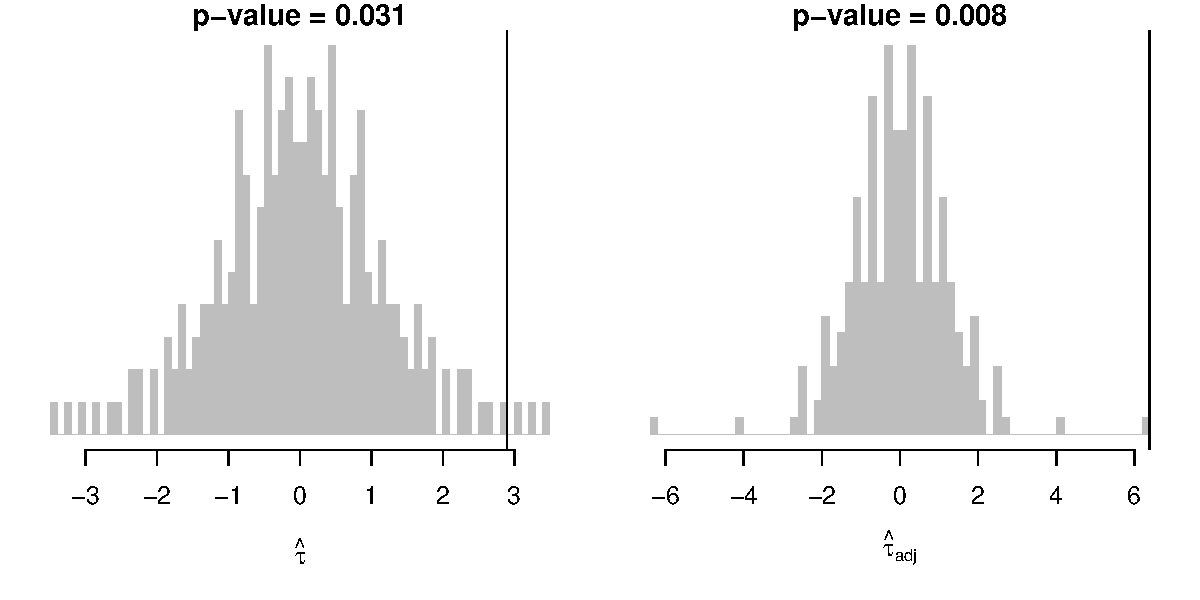
\includegraphics[width = \textwidth]{figures/frt_television.pdf}
\caption{Exact randomization distributions of the studentized statistics in Section \ref{sec::neyman-television-mpe} }\label{fig::frt-television-mpe}
\end{figure}



\section{Comparing the MPE and CRE}
\label{sec::discussion}

\citet{imai2008variance} compared the MPE and CRE. Heuristically, the conclusion is that the MPE gives more precise estimators if the matching is well done and the covariates are predictive of the outcome. However, without the outcome data in the design stage, it is hard to decide whether this is true or not. In the FRT, if covariates are predictive of the outcome, the MPE usually gives more powerful tests compared with the CRE. \citet{greevy2004optimal} illustrated this using simulation based on the Wilcoxon sign-rank statistic. However, this can be a subtle issue with finite samples. Consider an experiment with $2n$ units, with $n$ units receiving the treatment and $n$ units receiving the control. If we test the sharp null hypothesis at level $0.05$, then in the MPE, we need at least $2\times 5=10$ units since the smallest $p$-value is $1/2^5 = 1/32 < 0.05$ but $1/2^4 = 1/16 > 0.05$, but in the CRE, we need at least $2\times 4 = 8$ units since the smallest $p$-value is $1/\binom{8}{4} = 1/70 < 0.05$ but $1/\binom{6}{3} = 1/20 = 0.05$. So with $8$ units, it is impossible to reject the sharp null hypothesis in the MPE but it is possible in the CRE. Even if the covariates are perfect predictors of the outcome, the MPE is not superior to the CRE based on the FRT. 



\section{Extension to the general matched experiment}\label{sec::general-matched-experiment}

It is straightforward to extend the MPE to the general matched experiment with varying numbers of control units. Assume that we have $n$ matched sets indexed by $i=1, \ldots, n$. For the matched set $i$, we have $1+M_i$ units. The $M_i$'s can vary. The total number of experimental units is $N = n + \sum_{i=1}^n M_i$. 
Let $ij$ index the unit $j$ within matched set $i$ ($i=1,\ldots, n$ and $j=1,\ldots, M_i+1$). Unit $ij$ has potential outcomes $Y_{ij}(1)$ and $Y_{ij}(0)$ under the treatment and control, respectively. 


Within the matched set $i$ $(i=1, \ldots, n)$, the experimenter randomly selects exactly one unit to receive the treatment with the rest $M_i$ units receiving the control.
This general matched experiment is also a special case of the SRE with $n$ strata of size $1+M_i$ $(i=1, \ldots, n)$. 
Let $Z_{ij}$ be the treatment indicator for unit $ij$, which reveals one of the potential outcomes as
$$
Y_{ij} = Z_{ij} Y_{ij}(1) + (1-Z_{ij}) Y_{ij}(0) . 
$$ 

The average causal effect within the matched set $i$ equals
$$
\tau_i = (M_i + 1)^{-1} \sum_{j=1}^{1+M_i} \{ Y_{ij}(1)-Y_{ij}(0) \}. 
$$
Since the general matched experiment is a SRE, an unbiased estimator of $\tau_i $ is 
$$
\hat \tau_i = \sum_{j=1}^{M_i + 1} Z_{ij} Y_{ij} - M_i^{-1} \sum_{j=1}^{M_i+1} (1-Z_{ij}) Y_{ij}
$$
which is the difference in means of the outcomes within matched set $i$. 

Below we discuss the statistical inference with the general matched experiment. 


\subsection{FRT}

As usual, we can always use the FRT to test the sharp null hypothesis
$$
\HF: Y_{ij}(1) = Y_{ij}(0)  \text{ for all }  i=1,\ldots, n; j=1,\ldots, M_i+1. 
$$
Because the general matched experiment is a special case of the SRE with many small strata, we can use the test statistics defined in Examples \ref{eg::hodgeslehmann}, \ref{eg::ks-stratified}, \ref{eg::mpe-sign-rank}, \ref{eg::mpe-ksstatistics}, \ref{eg::mpe-sign}, as well as the estimators and the corresponding $t$-statistics from the following two subsections. 



\subsection{Estimating the average of the within-strata effects}


We first focus on estimating the average of the within-strata effects: 
$$
\tau = n^{-1} \sumn \tau_i .
$$
It has an unbiased estimator 
$$
\hat\tau = n^{-1} \sumn \hat \tau_i . 
$$
Interestingly, we can show that Theorem \ref{thm::varianceest-mp} holds for the general matched experiment, and so are other results for the MPE. In particular, we can use the OLS fit of the $\hat \tau_i $'s on the intercept to obtain the point and variance estimators for $\tau$. With covariates, we can use the OLS fit of the $\hat \tau_i $'s on the intercept and the $\hat\tau_{X,i}$'s, where
$$
\hat \tau_{X,i} = \sum_{j=1}^{M_i + 1} Z_{ij} X_{ij} - M_i^{-1} \sum_{j=1}^{M_i+1} (1-Z_{ij}) X_{ij}
$$
is the corresponding difference in means of the covariates within matched set $i$. 



\subsection{A more general causal estimand}


Importantly, the $\tau$ above is the average of the $\tau_i$'s, which does not equal the average causal effect for the $N$ units in the experiment when the $M_i$'s vary. The average causal effect equals
$$
\tau' = N^{-1} \sumn \sum_{j=1}^{1+M_i} \{ Y_{ij}(1)-Y_{ij}(0) \} = \sumn \frac{1+M_i}{N} \tau_i.
$$ 
To unify the discussion, I consider the weighted causal effect
$$
\tau_w =  \sumn w_i \tau_i
$$
with $\sumn w_i = 1$, 
which includes $\tau$ as a special case with $w_i = n^{-1}$ and $\tau'$ as a special case with $w_i = (1+M_i)/N $ for $i=1,\ldots, n$. It is straightforward to obtain an unbiased estimator 
$$
\hat\tau_w =  \sumn w_i \hat\tau_i,
$$
and calculate its variance 
$$
\var(\hat\tau_w ) = \sumn w_i^2 \var (\hat\tau_i ). 
$$
However, estimating the variance of $\hat\tau_w $ is quite tricky because the $\hat\tau_i$'s are independent random variables without any replicates. This is a famous problem in theoretical statistics studied by \citet{hartley1969variance} and \citet{rao1970estimation}. \citet{fogarty2018mitigating} also discussed this problem without recognizing these previous works. I will give the final form of the variance estimator without detailing the motivation:
$$
\hat{V}_w = \sumn c_i (\hat\tau_i -\hat\tau_w )  ^2
$$
where 
$$
c_i = \frac{    \frac{w_i^2}{1-2w_i}   }{   1 + \sumn  \frac{w_i^2}{1-2w_i} }.
$$
As a sanity check, $c_i $ reduces to $ \{  n(n-1) \}^{-1}$ in the MPE with $M_i=1$ and $w_i = n^{-1}$. For simplicity, we focus on the case with $w_i < 1/2$ for all $i$'s, that is, there is no matched set containing more than half of the total weights. The following theorem extends Theorem \ref{thm::varianceest-mp}.  

\begin{theorem}
\label{thm::hadamdard-matched-experiment}
Under the general matched experiment with varying $M_i$'s, if $w_i < 1/2$ for all $i$'s, then  
 $$
 E(\hat{V}_w ) - \var( \hat\tau_w  ) = \sumn c_i (\tau_i - \tau_w )^2 \geq \var( \hat\tau_w  )  \geq 0
 $$
with equality holding if the $\tau_i $'s are constant. 
\end{theorem}

Although the theoretical motivation for $\hat{V}_w $ is quite complicated, it is not too difficult to verify Theorem \ref{thm::hadamdard-matched-experiment} directly. I relegate the proof to Problem \ref{para::variance-general-matched}. 
 



\section{Homework Problems}

\paragraph{The true variance of $\hat{\tau}$ in the MPE}
\label{para::variance-mp-design}

Express $\var(\hat{\tau})$ in terms of the finite-population variances of the potential outcomes. 

\paragraph{A covariance estimator}\label{para::covariance-est-proof}
Prove Theorem \ref{thm::covariance-mp}.

\paragraph{Variance estimators via OLS}\label{para::seols-matchedpairs}
Prove Propositions \ref{prop::mpe-variance} and \ref{prop::colin2018regression}. 


\paragraph{Point and variance estimator with binary outcome}\label{para::binary-matchedpairs-neyman}


This problem extends Example \ref{eg::mcnenar-test-binary} to Neymanian inference. 

Express $\hat\tau$ and $\hat V$ in terms of the counts in Table \ref{tb::binarymatchedpairs}. 




\paragraph{Minimum sample size for the FRT}
\label{prob::minimum-n-0.001}

Extend the discussion in Section \ref{sec::discussion}.  Consider an experiment with $2n$ units, with $n$ units receiving the treatment and $n$ units receiving the control, and test the sharp null hypothesis at level $0.001$. What is the minimum value of $n$ for an MPE so that the smallest $p$-value does not exceed than $0.001$, and what is the corresponding minimum value of $n$ for a CRE?
 

\paragraph{Re-analyzing Darwin's data}

 
Chapter \ref{sec::frt-darwin-mpe} analyzed Darwin's data using the FRT based on the test statistic $\hat{\tau}$.

Re-analyze this dataset using the FRT with the Wilcoxon sign-rank statistic.

Re-analyze this dataset based on the Neymanian inference: report the unbiased point estimator, conservative variance estimator, and 95\% confidence interval.

\paragraph{Re-analyzing children's television workshop experiment data}

Chapter \ref{sec::neyman-television-mpe} analyzed the data from based on Neymanian inference.

Re-analyze this dataset using the FRT with different test statistics. 

Re-analyze this dataset using the FRT with covariate adjustment.




\paragraph{Re-analyzing \citet{angrist2009effects}'s data}\label{para::AL-mpe-neyman}

The original analysis of \citet{angrist2009effects}' was quite complicated. For this problem, please focus only on Table A1 of the original paper and view the schools as the experimental units. \citet{angrist2009effects} essentially conducted an MPE on the schools. Dropping pair 6 and all the pairs with noncompliance results in 14 complete pairs, with data shown below and also in \ri{AL2009.csv}: 
\begin{lstlisting}
   pair z  pr99  pr00  pr01  pr02
1     1 0 0.046 0.000 0.091 0.185
2     1 1 0.036 0.051 0.000 0.047
3     2 0 0.054 0.094 0.184 0.034
4     2 1 0.050 0.108 0.110 0.095
5     3 0 0.114 0.000 0.056 0.075
6     3 1 0.098 0.054 0.030 0.068
7     4 0 0.148 0.162 0.082 0.075
8     4 1 0.134 0.390 0.339 0.458
9     5 0 0.152 0.105 0.083 0.129
10    5 1 0.145 0.077 0.579 0.167
11    6 0 0.188 0.214 0.375 0.545
12    6 1 0.179 0.165 0.483 0.444
13    7 0 0.193 0.771 0.328 0.583
14    7 1 0.189 0.186 0.168 0.368
15    8 0 0.197 0.350 0.000 0.383
16    8 1 0.200 0.071 0.667 0.429
17    9 0 0.213 0.176 0.164 0.172
18    9 1 0.209 0.165 0.092 0.151
19   10 0 0.211 0.667 0.250 0.617
20   10 1 0.219 0.250 0.500 0.350
21   11 0 0.219 0.153 0.185 0.219
22   11 1 0.224 0.363 0.372 0.342
23   12 0 0.255 0.226 0.213 0.327
24   12 1 0.257 0.098 0.107 0.095
25   13 0 0.261 0.071 0.000    NA
26   13 1 0.263 0.441 0.448 0.435
27   14 0 0.286 0.161 0.126 0.181
28   14 1 0.285 0.389 0.353 0.309
\end{lstlisting}
The outcomes are the Bagrut passing rates in the years 2001 and 2002, with the Bagrut passing rates in 1999 and 2000 as pretreatment covariates. Re-analyze the data based on the Neymanian inference with and without covariates. In particular, how do you deal with the missing outcome in pair 25? 
% (1) using the FRT with and without covariate adjustment and (2) based on the Neymanian inference with and without covariates. In particular, how do you deal with the missing outcome? 
 
 
\paragraph{Variance estimation in the general matched experiment} 
 \label{para::variance-general-matched}

This problem contains more details for Section  \ref{sec::general-matched-experiment}. 
 
 
First, prove Theorem  \ref{thm::varianceest-mp} for the general matched experiment.
Second, prove Theorem \ref{thm::hadamdard-matched-experiment}. 
 
Remark: For the second part, we can first verify that $\hat\tau_i -\hat\tau_w$ has mean $\tau_i - \tau_w$ and variance
 $$
 \var(\hat\tau_i -\hat\tau_w) = \var(\hat\tau_w ) + (1-2w_i) \var(\hat\tau_i). 
 $$


\paragraph{Recommended readings}

\citet{greevy2004optimal} provided an algorithm to form matched pairs based on covariates. 
\citet{imai2008variance} discussed the estimation of the average causal effect without covariates,
and 
\citet{fogarty2018regression} discussed covariate adjustment in MPEs. 


